\documentclass[a4paper,french]{paper}
\usepackage{../../../../../_assets/latex/5N_OPTO_ELEC}

%Informations about this document 
%------------------------------------------
\def\module{Opto-Electronique - S5}
\def\moduleAbrege{5N-027-SCI / OptoElec}
\def\annee{2024-2025}

\def\titre{Séance 5 / Photodétection}
\author{Julien VILLEMEJANE}

\subtitle{Séance 5}
\institution{LEnsE / Institut d'Optique Graduate School}

\title{\titre}
\begin{document} 
%Beginning First Page. 
%------------------------------------------
\enteteThematiqueObligatoire{}

\textit{Pour ce TD, on pourra s'appuyer sur la fiche résumée} : \href{https://lense.institutoptique.fr/ressources/Annee1/Electronique/fiches/2020_FR_Diodes_LED.pdf}{Diodes / LED / Photodiodes}

%Beginning Content. 
%------------------------------------------

%%%%%%%%%%%%%%%%%%%
%%%%%%%%%%%%%%%%%%%
\encadreTDExo{5.1 - Emettre une information lumineuse}{
En se basant sur une \textbf{LED IR} de type SFH415.

Proposer un montage émetteur permettant d'obtenir un flux lumineux sinusoïdal sans risque pour la LED, et donner les paramètres des différentes sources utilisées et des autres éléments du montage.
}

%%%%%%%%%%%%%%%%%%%
%%%%%%%%%%%%%%%%%%%
\encadreTDExo{5.2 - Transmettre une information par la lumière}{
En se basant sur une \textbf{LED IR} de type SFH415 et une \textbf{photodiode} de type SFH229, on souhaite réaliser un système de transmission d'information par la lumière.

On se propose dans un premier temps d'utiliser le montage "simple" de photodétection.

\begin{center}
	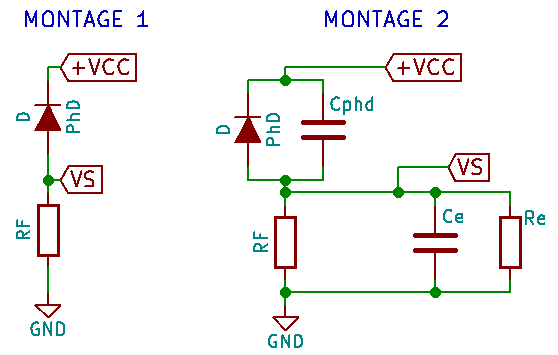
\includegraphics[width=7cm]{images/photodetection_simple_modele.png}
\end{center}

A quoi correspondent les deux montages proposés ?

Donner la fonction de transfert du montage en fonction du flux lumineux reçu.

Quelle est alors la limite en fréquence d'un tel montage ? Peut-on transmettre des données binaires ?
} 

%%%%%%%%%%%%%%%%%%%
%%%%%%%%%%%%%%%%%%%
\encadreTDExo{5.3 - Transmettre une information par la lumière - transimpédance}{
En se basant sur une \textbf{LED IR} de type SFH415 et une \textbf{photodiode} de type SFH229, on souhaite réaliser un système de transmission d'information par la lumière.

On se propose dans un premier temps d'utiliser le montage de photodétection de type transimpédance.

\begin{center}
	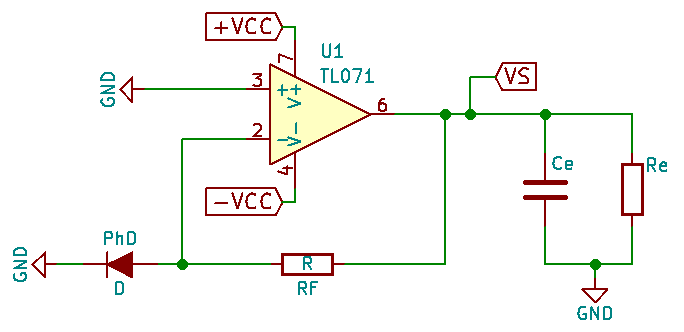
\includegraphics[width=8cm]{images/photodetection_transimpedance.png}
\end{center}

Donner la fonction de transfert du montage en fonction du flux lumineux reçu.

Quelle est alors la limite en fréquence d'un tel montage ? Peut-on transmettre des données binaires ?
}

%%%%%%%%%%%%%%%%%%%
%%%%%%%%%%%%%%%%%%%
\encadreTDExo{5.B1 - Modéliser le montage transimpédance}{
Dans l'exemple précédent, nous avons supposé l'amplificateur linéaire idéal. 

On prendra le modèle suivant pour l'amplificateur linéaire :

$$V_S = \frac{A_0}{1 + j \cdot \frac{\omega}{\omega_0}} \cdot (V^+ - V^-)$$

Calculer la fonction de transfert $T(j\cdot \omega) = V_S /  i_{PHD}$ du montage suivant :
} 


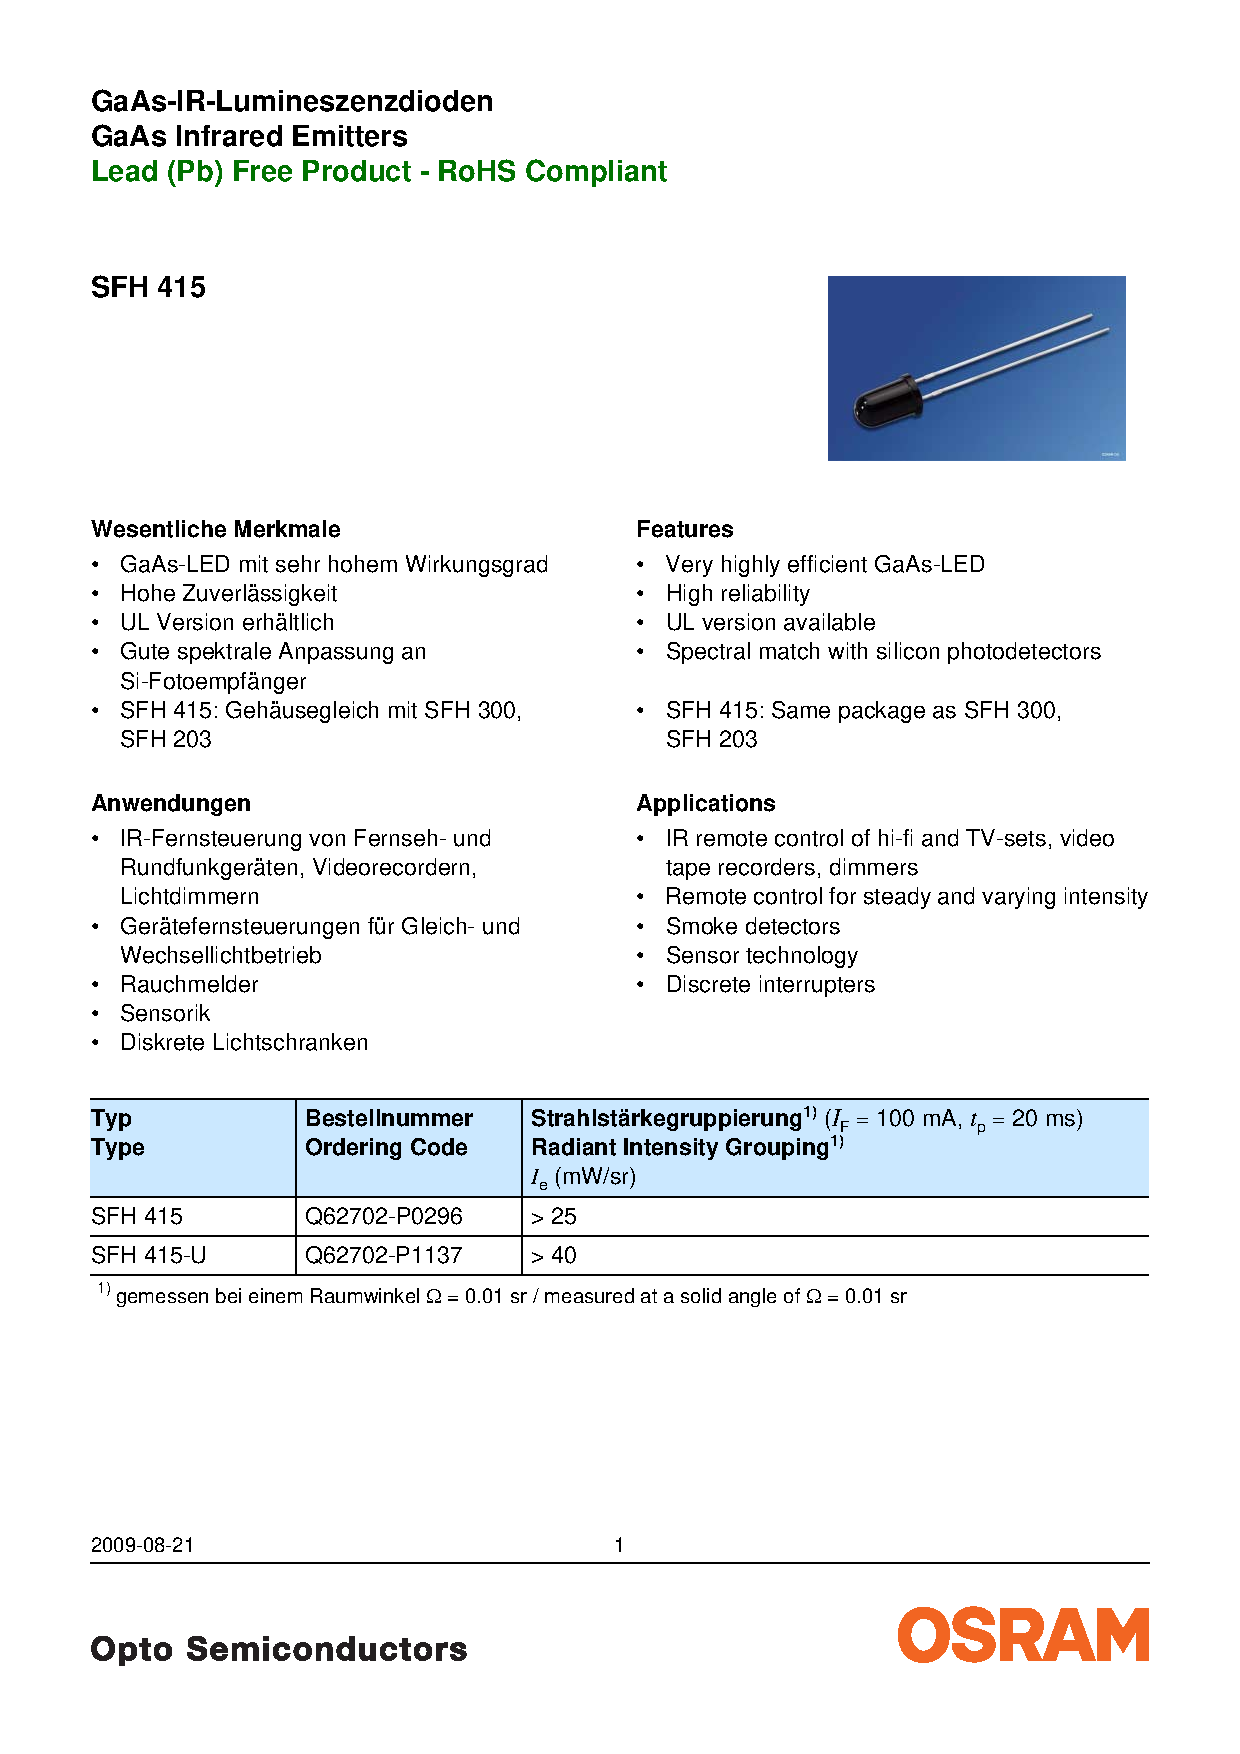
\includepdf[pages=1-3]{docs/SFH415.pdf}
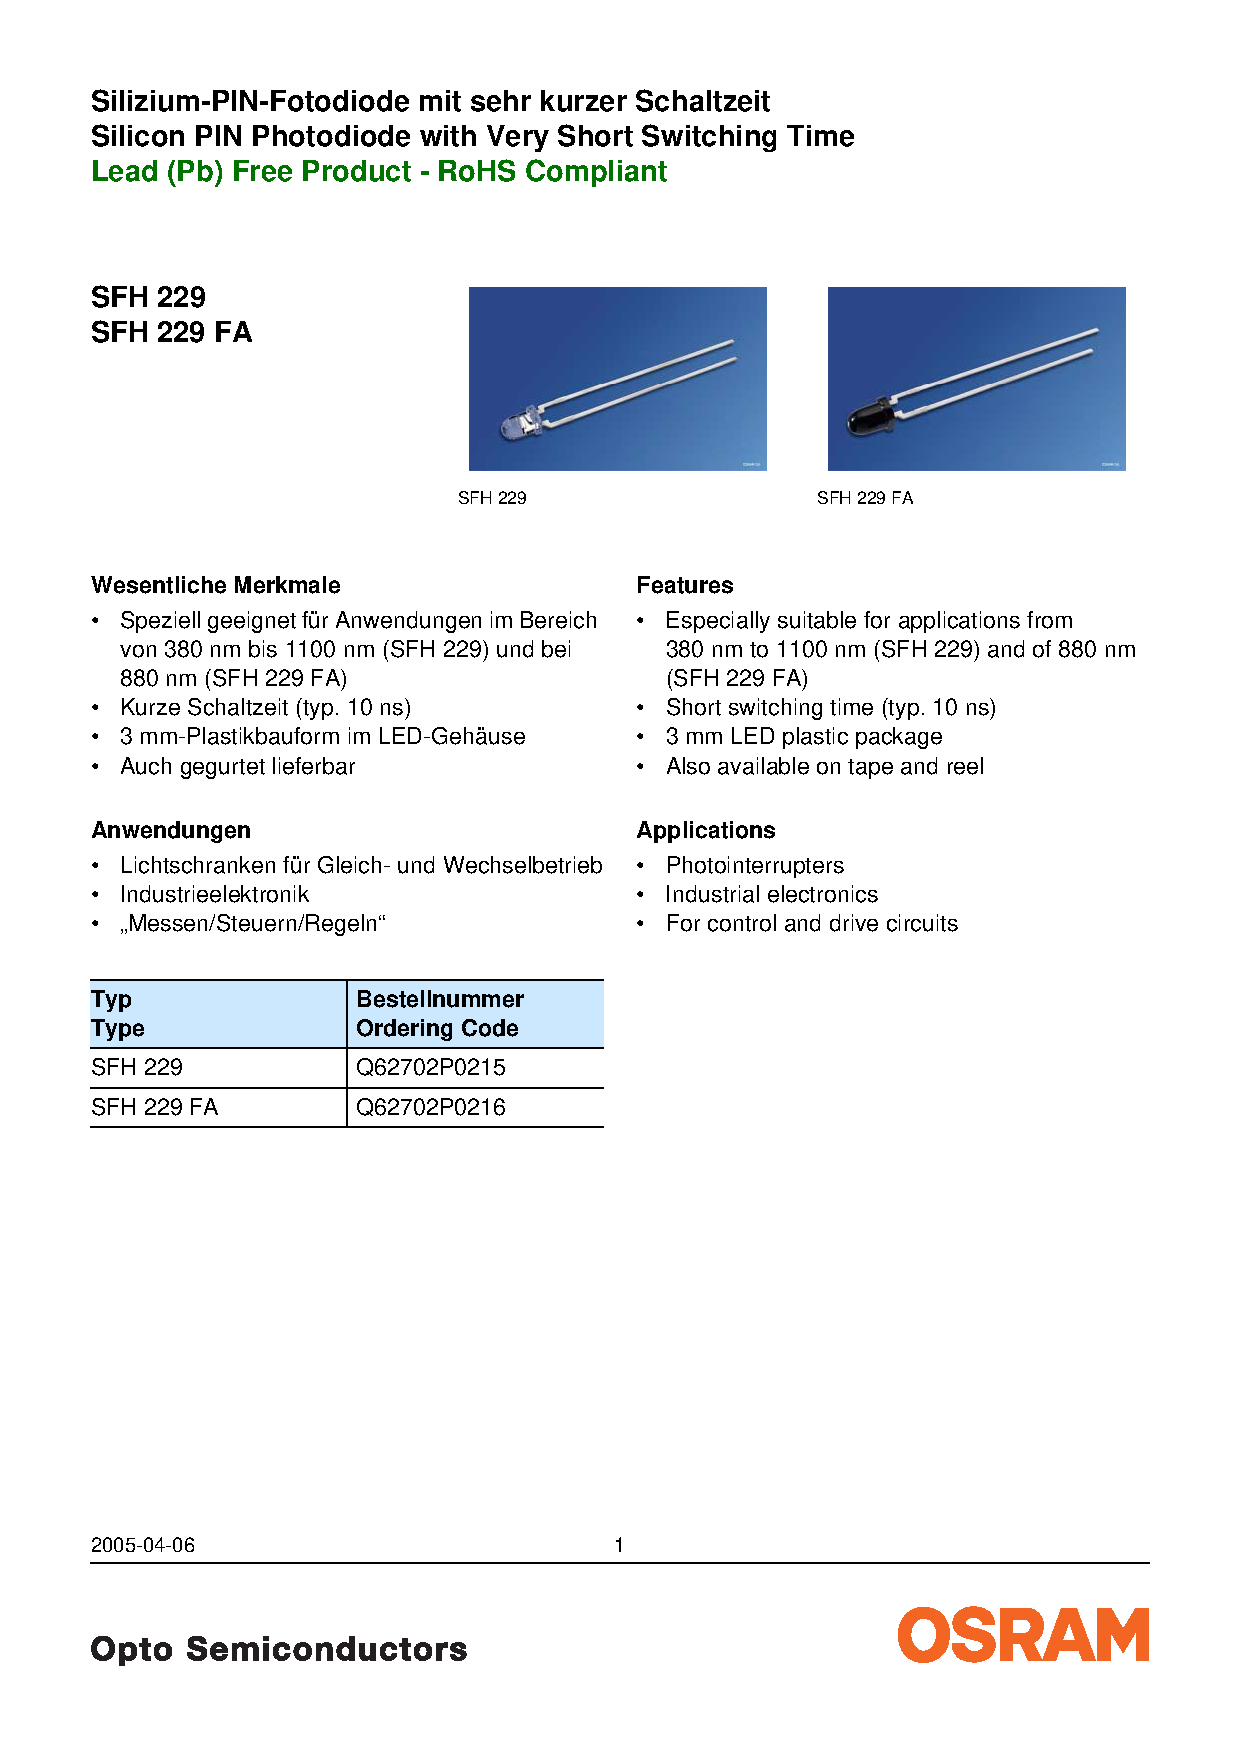
\includepdf[pages=1-5]{docs/SFH229.pdf}

\end {document}